\section{Introduction}
% \begin{figure}
%   \centering
%   \fbox{\rule[-.5cm]{0cm}{4cm} \rule[-.5cm]{4cm}{0cm}}
%   \caption{Sample figure caption.}
% \end{figure}
Online news portals such as BBC, CNN, and Bing News have a huge number 
of readers daily. Many of them are anonymous or logged in as guests who 
typically do not read many stories in a single login session.
Given the limited interactions users engage with the portals, it is often 
hard for the systems to fully understand the user behavior, posing significant challenges to recommendation systems. 

Conventional news recommendation approaches tend to formulate the 
recommendation task as CTR prediction task, and they mainly rely on 
collaborative filtering and factorization machine~\cite{cheng2016wide,guodeepfm2017,wang2018modeling,ge2020graph,hu2020graph,xie2020deep}, 
which requires the system to keep track of the user history 
and can not be applied to anonymous visits or guest logins. 
Recent neural approaches for news recommendation mostly focus on 
encoding the text feature of articles with 
attention mechanism~\cite{wang2018dkn,zhu2019dan,wu_neural_2019-1,wu2019npa,wang2020fine,wu2020CPRS} 
when modeling the user interest while paying little attention to the click 
behavior or the article-to-article transition. 
For example, they have not taken full advantage of the temporal information 
associated with the reading behavior, which is important
especially when the interactions with the user are sparse.

\begin{figure}[th]
    \centering
    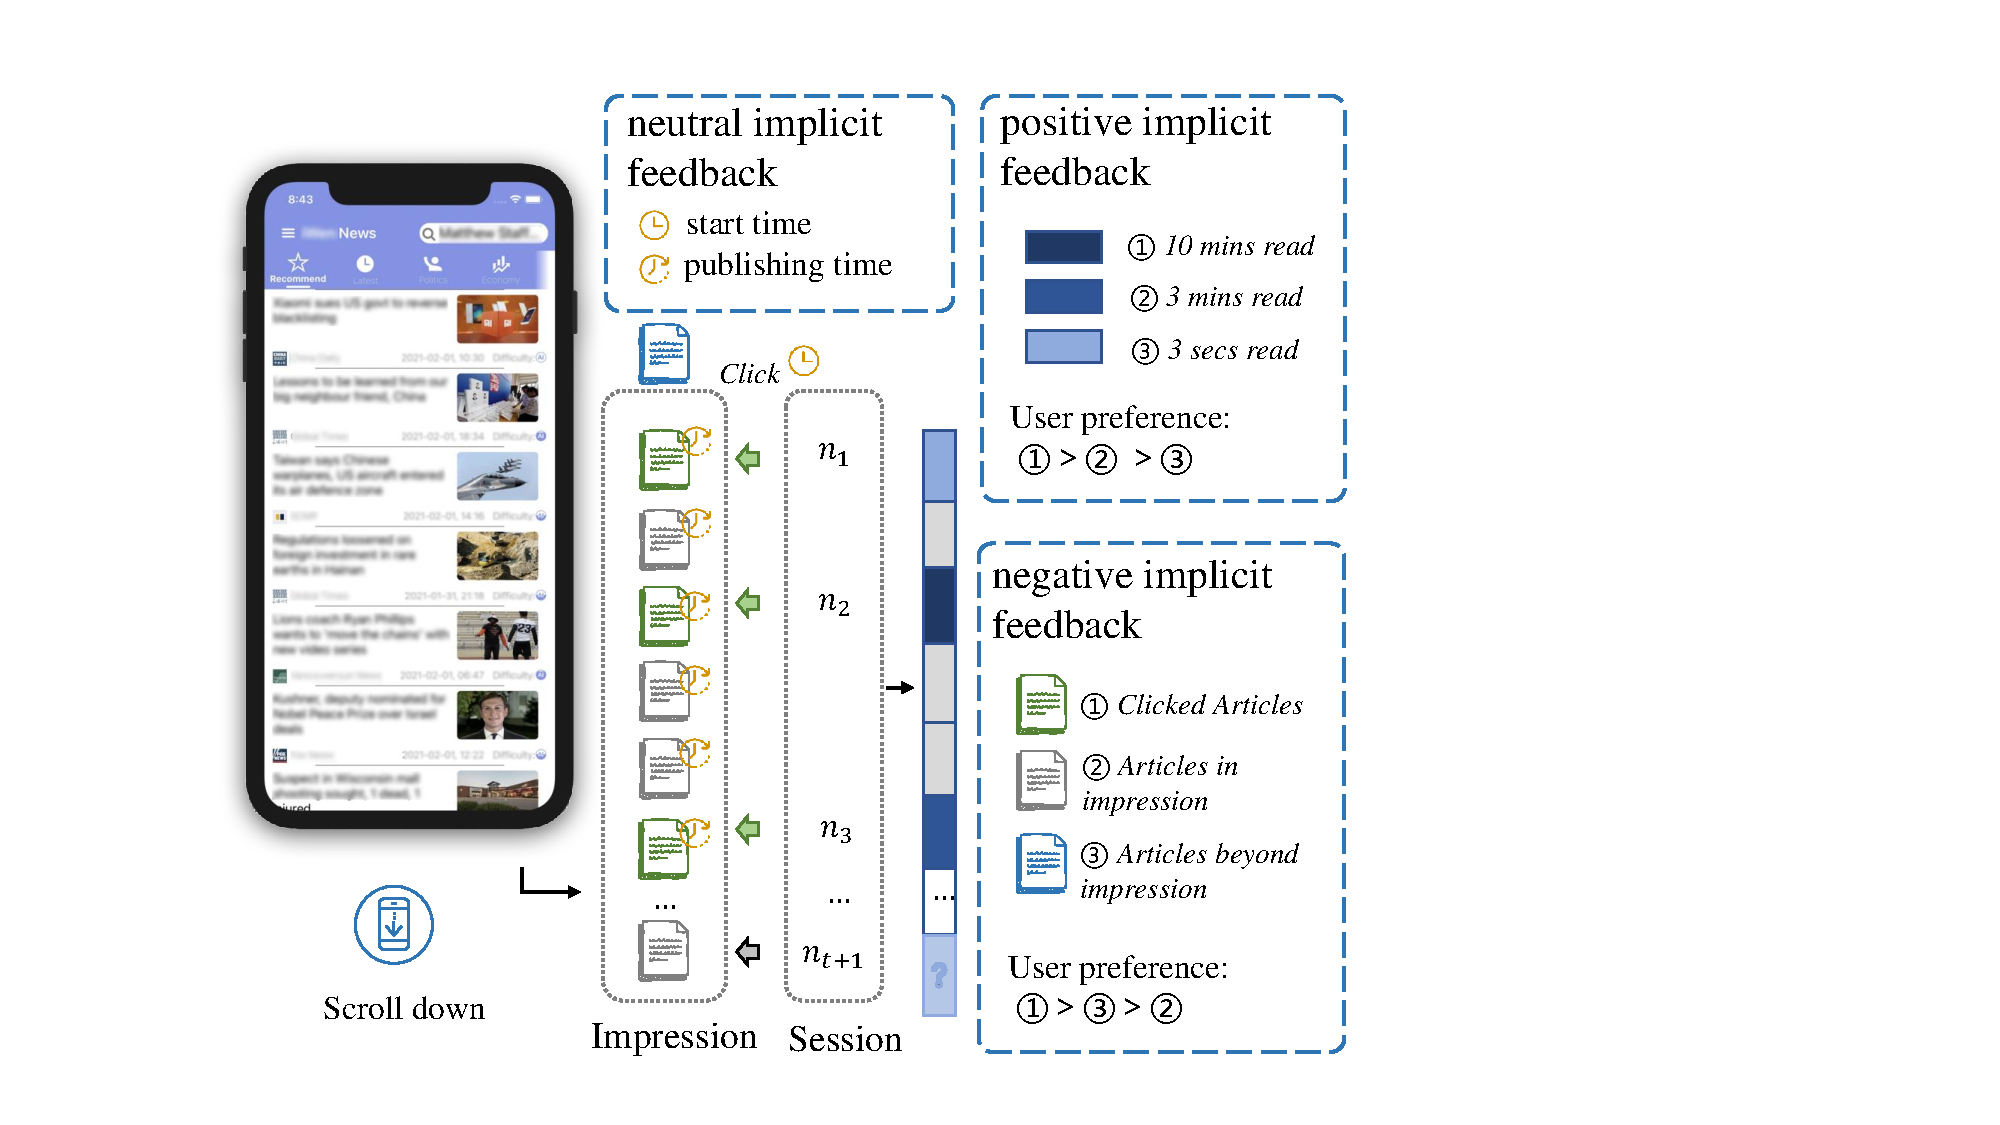
\includegraphics[width=\columnwidth]{fig/stream.pdf}
    \caption{A schematic of session-based news reading. 
    A user may spend different amounts of time on different clicked articles, 
representing different level of preference in an implicit form of 
\textbf{positive feedback}; 
an article that the user has an impression on but does not eventually click 
represents an implicit form of \textbf{negative feedback}; the start time of the click and publishing time of articles are formed as \textbf{neutral feedback}.}
\label{fig:session}
\end{figure}

Considering the above issues, it's natural and realistic to formulate the 
streaming-like news recommendation task for anonymous users as 
a session-based recommendation task~\cite{sottocornola2018session,gabriel2019contextual}. 
The task is to recommend the next item that the user might be interested 
in given the previous sequence of behaviors within a session, 
where a \textit{session} is usually 
a short period of time (e.g., 30 minutes) during which the user is logged on.
Session-based recommendation is widely used in the e-commerce or 
video streaming domain~\cite{xu2019time,pan2020star}, and can successfully capture
users' short-term intention transition process~\cite{epure_recommending_2017,symeonidis2020session}. However, they rarely consider the implicit feedback from user behaviors.

In this paper, we are interested in exploiting user actions outside the 
clicks themselves. We call them ``implicit feedback'', as
illustrated in \figref{fig:session}. 
Typical implicit feedback can be extracted from browsing the main page, 
reading an article, closing an article, backtracking~\cite{smadja_understanding_2019}, 
etc. We believe that modeling such implicit feedback ``explicitly'' 
in the session-based recommendation system 
can help the recommender understand user intention better. 
In this work, we focus on answering these questions:
\begin{itemize}
    \item If a user clicked an article, did she really \textit{like} it? 
    \item If a user did not click an article, did she \textit{dislike} it?
    \item How do we model the temporal characteristics of the user and the articles in 
the system?
\end{itemize}

First, in traditional recommendation systems, ``clicks'' usually indicate a ``like'' or a
vote from the user, but things are a bit different for news reading. 
Users may be ``tricked'' into clicking an article~\cite{wang2020click} 
and once they realize that, they will quickly back out and switch to other articles. 
Thus the time a user spends on reading an article is a better, finer-grained 
gauge of the user's preference for the article~\cite{wu2020CPRS}, than 
just the click alone, which is only binary. We model this as the \textbf{implicit 
positive feedback} in this paper. 

Second, just because the user did not click on an article does not necessarily
mean the user does not like it; maybe she was never exposed to this article!  
We can infer what articles might have an impression~\cite{xie2020deep} on 
the user during a session by by assuming that articles are presented to the user 
roughly in the order of their publication time. 
Only those articles within her list of impressions but not clicked are considered
``not interesting'' to her. This is called \textbf{implicit negative feedback}.

Finally, while the positive and negative feedback helps us estimate the 
connection between the user and articles, 
some critical temporal information is useful to model
the user and the articles individually. 
The session start time of a user may suggest
the daily routine of that user. We can expect users who read on
the same day of a week or same time of a day to have to
share the same reading behavior or even background.
On the other hand, the publishing time of each article can also be
formed into a sequence in a session, which reflects the user's sensitivity of 
the timeliness of the stories. We thus carefully design the representation of
session start time and article publishing time as 
\textbf{implicit neutral feedback}.


In this paper, we formulate a session-based recommendation task to 
predict the next possible article 
in each session from the candidate articles pool. Our main contributions are:
\begin{itemize} 
\item For the first time, we leverage the positive/negative/neutral implicit feedback 
in anonymous session-based news recommendation (\secref{sec:approach});
\item We design novel representations for temporal information 
and incorporate it with positive and negative feedback 
into a deep attention network;
\item Our comprehensive offline evaluations on three real-world datasets 
show the clear advantage of our proposed method in terms of overall performance on 
diversity, accuracy and serendipity in both normal and 
cold-start scenarios (\secref{sec:experiment}).
\end{itemize}
% This paper makes the following contributions: 
% \begin{itemize}
%     \item To the best of our knowledge, we are the first to leverage the positive/negative implicit feedback in anonymous session-based news recommendation;
%     \item Our method is very simple and can be easily plugged into other approaches.
%     \item Our comprehensive experiments on three real-world datasets show the promising performance and better trades off the dilemma between 
% diversity and accuracy. 
% \end{itemize}
